\section{Path Planner}

In an attempt to better track the ground path with regards to the camera, a simple path planner will be developed. The goal of the path planner is to alter the position of the aircraft so that the camera will be focused on the point of interest on the ground, regardless of the attitude of the aircraft. The path will first be generated as a Dubins path that later will be altered with regards to the kinematic model developed in chapter \ref{ch:kinematics}.


\subsection{Dubin's Path}
\label{ch:dubins_path}

As already presented in chapter \ref{ch:path_literature}, a Dubin's path consists of two circular arcs connected by a straight line \cite{DUBIN}. The path generated here will only be in two dimensions, as it is assumed that the aircrafts autopilot will maintaint a constant height. In order for a vehicle to follow a Dubins path, it must be possible to describe the kinematics of the vehicle as a Dubins vehicle \cite{dubinYONG}:

\begin{subequations}
\begin{equation}
	\dot{x}(t) = cos(\theta(t))u_1(t)
\end{equation}
\begin{equation}
	\dot{y}(t) = sin(\theta(t))u_1(t)
\end{equation}
\begin{equation}
	\dot{\theta}(t) = u_2(t)
\end{equation}
\end{subequations}

where $u_1$ is the linear velocity, $u_2$ is the angular velocity and $\theta$ is the heading angle. For the kinematic model of the aircraft in this paper, $u_1$ equals to $V$, $\theta$ equals to $\psi$.

\begin{figure}[!ht]
    \centering
    \makebox[\textwidth][c]{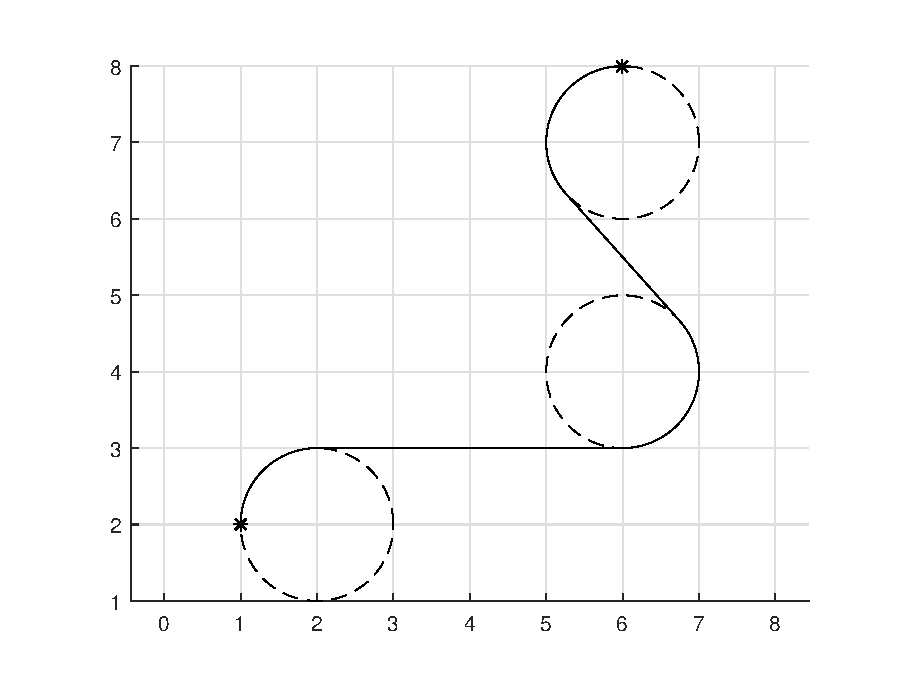
\includegraphics[width=\textwidth, keepaspectratio=true]{dubins_example.eps}}
    \caption{Illustration of a simple Dubins path.}
	\label{fig:dubins_example}
\end{figure}

When generating a Dubins path there are foure cases that need to be taken into consideration \cite{suaBEARD}. Depending on the start and end configuration a Dubins path can either start and end with a circle that the vehicle traces either clockwise or counterclockwise, and the four cases are the different combinations of start and end circle.

In order to generate a Dubins path for this paper the algorithm proposed in Beard \& McLain was used (algorithm 7, \cite{suaBEARD}). The algorithm takes the start and end postion, start and end heading and radius of the circles as input. Based on these parameters the algorithm calculates the length of the path created by any of the four cases, and the case that gives the shortest path length is chosen. The outputs of the algorithm is the length of the path together with other parameters describing the path. The parameters that are calculated by the algorithm are shown in \ref{fig:dubins_algorithm}.

\begin{figure}
	\import{/}{path_algo.tex}
	\caption{Illustration of the parameters returned by the Dubins algorithm.}
	\label{fig:dubins_algorithm}
\end{figure}

The algorithm that generates the Dubins path only generates the path between two points, hence another algorithm is needed in order to generate the Dubins path involving several waypoints. For this another algorithm by Beard \& McLain (algorithm 8, \cite{suaBEARD}) was used. This algorithm takes a list of waypoints together with the position of the aircraft and the desired turning radius as input. Based on the inputs the algorithm generates a Dubins path and then calculates where on the path the aircraft is. It returns information about whether or not the aircraft should follow a straight line or track a circle, and the information needed to do this. This information is given to two algorithms that calculate the desired heading that can be fed to the autopilot. These algorithms will be described in chapter \ref{ch:path_follower}.


\subsection{Altering the original path}

The Dubins path described in the previous section will be used to generate a path based on the initial waypoints that the UAV is to observe. The problem with this path is that it will tell the aircraft to turn when it is just above the ground path, and the roll used to turn will cause the fixed camera to lose the points of interest from its field of view. 

In order to compensate for the roll of the aircraft, the Dubins path will be altered so that the camera is always pointing at the points of interest. The principle is shown in figure \ref{fig:altered_path}. 

\begin{figure}[!ht]
    \centering
    \makebox[\textwidth][c]{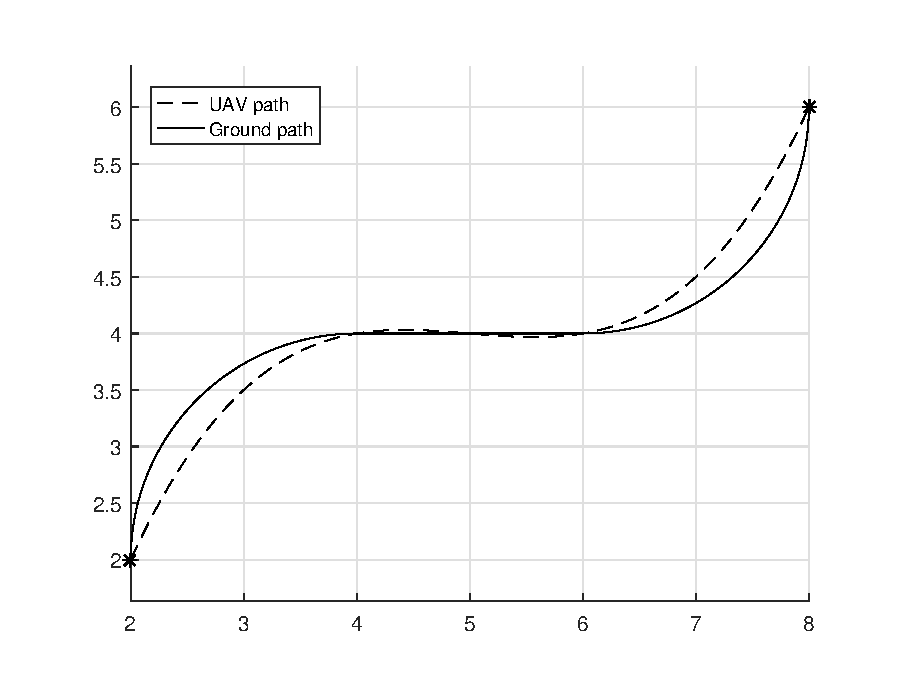
\includegraphics[width=\textwidth, keepaspectratio=true]{altered_path.eps}}
    \caption{Illustration of the principle for altering the path.}
	\label{fig:altered_path}
\end{figure}

In order to compensate the roll the kinematic model developed in \ref{ch:kinematics} can be used. For altering the path only the distance from the aircraft frame \{b\} to the camera point caused by the roll is needed. This corresponds to $c_{y/b}^b$ from equation (\ref{eq:camera_pos}):

\begin{equation}
	c_{y/b}^b = z_ntan(\phi).
\end{equation}

$c_{y/b}^b$ only represents the distance the path is to be moved, and not the direction. The direction the path is to be moved is given by the heading $\psi$, and the direction should be perpendicular to $\psi$ as shown in figure \ref{fig:path_alter_dir}. The coordinates for the new path $\bm{p}_d$ in the body frame \{b\} then becomes

\begin{equation}
	\bm{p}_{b,d} =
	\begin{bmatrix}
		x_{b,d} \\ y_{b,d}
	\end{bmatrix}
	=
	\begin{bmatrix}
		c_{y/b}^b sin(\psi) \\
		-c_{y/b}^b cos(\psi)
	\end{bmatrix},
\end{equation}

and in the NED frame \{n\}:

\begin{equation}
	\bm{p}_{n,d} = \bm{p}_{b/n}^n + \bm{p}_{b,d}.
\end{equation}

\begin{figure}[!ht]
    \import{/}{path_alter.tex}
    \caption{Illustration of the direction for altering the path.}
	\label{fig:path_alter_dir}
\end{figure}